\documentclass[article,12pt,onesidea,4paper,english,brazil]{abntex2}

\usepackage{lmodern, indentfirst, nomencl, color, graphicx, microtype, lipsum}			
\usepackage[T1]{fontenc}		
\usepackage[utf8]{inputenc}		

\setlrmarginsandblock{2cm}{2cm}{*}
\setulmarginsandblock{2cm}{2cm}{*}
\checkandfixthelayout

\setlength{\parindent}{1.3cm}
\setlength{\parskip}{0.2cm}

\SingleSpacing

\begin{document}
	
	\selectlanguage{brazil}
	
	\frenchspacing 
	
	\begin{center}
		\LARGE \MakeUppercase{Análise de indicadores institucionais do IFRO de 2009 a 2015}
		
		\normalsize
		Julian Alves de Queiroz \,\, 
		Rosa Martins Costa Pereira\footnote{Orientadora} \\
		Gilberto Paulino da Silvar\footnote{Coorientador} 
		Álvaro Victor Oliveira\footnote{Estudante/Campus Porto Velho Calama} 
	\end{center}
	
	% resumo em português
	\begin{resumoumacoluna}
		Essa pesquisa teve como objetivos analisar indicadores de desempenho acadêmico do IFRO
		no período de 2009 a 2015, sistematizar indicadores de eficácia, eficiência, evasão e retenção dos
		cursos técnicos e de graduação (modalidade presencial) do IFRO no período de 2009 a 2015,
		elaborar tabelas a partir de dados primários extraídos de sistemas,
		elaborar relatório por indicador, produzir relatório final com análise dos indicadores definidos
		para a pesquisa e calculados pelas instituições da Rede Federal de EPCT em cumprimento aos
		Acórdãos do Tribunal de Contas da União. As atividades desenvolvidas neste plano de trabalho
		consistiram na realização da extração de dados de todos os \textbf{cursos superiores do IFRO} ofertados
		no período estudado (2009 – 2015), seleção dos cursos com ciclos de matrícula na situação
		“concluídos”, elaboração de planilhas modelo, realização de cálculos por indicador para cada
		curso e campus, finalização das planilhas, sistematização de dados e elaboração de relatório final.
	\end{resumoumacoluna}
	
	\section*{Introdução}
	
	Planejar, de forma estratégica, envolve tanto o diagnóstico quanto o monitoramento e
	tomada de decisão das realidades que se deseja transformar. Nesse sentido, as instituições de
	ensino precisam criar mecanismos para conhecer as demandas sociais e os diferentes cenários que
	interferem ou podem interferir no planejamento da oferta ou redimensionamento de seus cursos.
	
	O levantamento de dados educacionais é importante para traçar um perfil da instituição,
	conhecer seus pontos fortes e limitações, gerando indicadores acadêmicos que forneçam aos
	gestores informações imprescindíveis ao processo de tomada de decisões e servindo de subsidio
	para a formulação de políticas públicas na área da educação.
	
	Espera-se que este estudo possibilite a fácil visualização e a reflexão de indicadores
	acadêmicos do IFRO no período de 2009 a 2015 que podem ser utilizados pela instituição para
	nortear as ações e dispositivos das políticas institucionais, dentre elas, o planejamento da
	distribuição de recursos, a autorização para criação de novos cursos ou seu redimensionamento e
	até mesmo contribuir com os gestores em seus processos administrativos decisórios.
	
	\section*{Material e Método}
	
	Os materiais utilizados para o desenvolvimento da pesquisa são as informações disponíveis
	no Plano de Desenvolvimento Institucional (PDI) do IFRO e as disponíveis no Sistema de
	gerenciamento de matriculas da Rede Federal (SISTEC).
	
	O procedimento metodológico principal foi a extração de dados e construção de tabelas
	contendo os indicadores. Os relatórios de indicadores foram gerados de forma padronizada, pela
	extração centralizada no MEC e posteriormente, validados com os dados do IFRO. Atendendo
	recomendações do TCU, a SETEC extrai os dados brutos do SISTEC, SIAPE e SIAFI, sistemas
	oficiais de registro de matriculas, de gestão de pessoas e movimentação financeira,
	respectivamente. A partir de dados primários extraídos na mesma data por indicadores, serão
	realizados procedimentos de cálculo automatizados dos componentes, para então gerar as
	informações dos indicadores, ganhando consistência nos resultados consolidados.
	
	A pesquisa foi quali-quanti. Essa abordagem é escolhida quando os pesquisadores desejam
	realizar um estudo que seja, ao mesmo tempo, histórico e de característica cientifico
	generalizável, pela busca da existência de padrões no decorrer de um determinado período de
	tempo.
	
	A apresentação, pura e simples do indicador, sem a devida analise, será tomada como
	descumprimento das determinações dos acórdãos TCU, ensejando sanções da SETEC as
	instituições da Rede Federal de EPCT, que serão arroladas no processo de análise do Relatório de
	Gestão da SETEC.
	
	A análise teve como pressuposto a orientação do Manual para Produção e Analise dos
	Indicadores da Rede Federal de EPCT (Brasil, 2015), segundo a qual, dentro do possível, cada
	indicador deverá ser analisado levando em consideração seus aspectos:
	
	1 - Temporal: deverão ser comparados os valores dos índices em diferentes anos, possibilitando
	verificar se os mesmos estão avançando na direção desejada;
	
	2 – Nível de agregação: a análise deverá contemplar os dados no maior nível de agregação (por
	IF) e ainda envolver sua estratificação em nível de campus, eixo tecnológico, tipo de curso e etc.,
	quando necessário;
	
	3 – Categorias de Aplicação: os indicadores podem ser agrupados nos quatro aspectos da ação
	educativa: capacidade de oferta de vagas (a e b); eficiência e eficácia (c, d e h); adequação da
	força de trabalho docente (f e g); adequação do orçamento atribuído a instituição (i, j e k);
	
	4 – Outros: além dos aspectos anteriores, a instituição deverá, a partir dos dados, elaborados
	analises que contemplem suas especificidades. A partir das análises de cada indicador a
	instituição deverá explicitar as ações a serem adotadas para uma melhoria continua dos
	indicadores institucionais.
	
	Nesta pesquisa foram utilizados cinco indicadores de desempenho institucional e acadêmico,
	são eles:
	
	\subsection*{Descrição dos Indicadores}
	\textbf{Indicador 1: RELAÇÃO CANDIDATOS POR VAGA (RCV):} Este indicador mede a
	consonância entre a oferta de vagas em relação à procura do público pelos cursos ofertados.
	
	A fórmula utilizada para efetuar o cálculo do indicador é:
	
	\textbf{RCV=INGRESSANTES/(VAGAS OFERTADAS PARA INGRESSO) X 100.}
	
	\textbf{Indicador 2: RELAÇÃO DE INGRESSO POR MATRÍCULA ATENDIDA (RIM):} Este
	indicador mede a capacidade de renovação do quadro discente.
	
	A fórmula utilizada para efetuar o cálculo do indicador é:
	
    \textbf{	RIM=INGRESSANTES/MATRICULAS ATENDIDAS X 100.}
	
	\textbf{Indicador 3: RELAÇÃO DE CONCLUINTES POR MATRÍCULA ATENDIDA (RCM):}
	Esse indicador mede do total dos alunos matriculados, quantos concluíram o curso no tempo
	previsto. Ele mensura a capacidade de alcançar êxito escolar.
	
	A fórmula utilizada para efetuar o cálculo do indicador é:
	
	\textbf{RCM=CONCLUINTES/(MATRICULAS ATENDIDAS) X 100}.
	
	\textbf{Indicador 4: EFICIÊNCIA ACADÊMICA DE CONCLUINTES (EAC):} esse indicador mede
	a relação entre todos os alunos que concluíram o curso no período previsto e todos que de alguma
	forma finalizaram o curso (desistências/evasões/trancamentos/transferências e desligamentos).
	
	A fórmula utilizada para efetuar o cálculo do indicador é:
	
	\textbf{RCM=CONCLUINTES/(MATRICULAS ATENDIDAS) X 100.}
	
	\textbf{Indicador 5: RETENÇÃO DO FLUXO ESCOLAR:} esse indicador mede a relação de alunos
	que não concluíram o curso no tempo previsto.
	
	A fórmula utilizada para efetuar o cálculo do indicador é:
	RFE=RETIDOS/(MATRICULAS ATENDIDAS) X 100.
	
	\section*{Resultados}
	
	Para começar a falar sobre os resultados obtidos na pesquisa devemos, primeiramente,
	abordar a relação dos cursos do IFRO com cada indicador para melhor compreensão dos
	resultados encontrados.

	Nesse estudo, apresentamos os resultados por amostragem. Para cada indicador,
	selecionamos um curso vinculado a um campus do IFRO. Após a análise detalhada de cada
	indicador, apresentaremos uma análise geral de todos os cursos da instituição por indicador com o
	objetivo de contribuir para a compreensão sistêmica dos resultados e para a auto-avaliação
	institucional.
	
	O indicador 1 mostra a relação candidato por vaga, este indicador mede a consonância
	entre a oferta de vagas em relação à procura do público. Exemplo desse indicador é o resultado
	encontrado no curso de Licenciatura em Biologia no Campus Ariquemes onde nos 3 (três)
	primeiros anos do curso a procura chegou a 1,23 candidatos por vagas ofertadas, em seguida,
	houve uma queda em quase 0,13 \% se comparado aos anos anteriores, contudo manteve-se a
	procura acima da quantidade de vagas ofertadas nesse campus.
	
	\begin{figure}[ht]
		\centering
		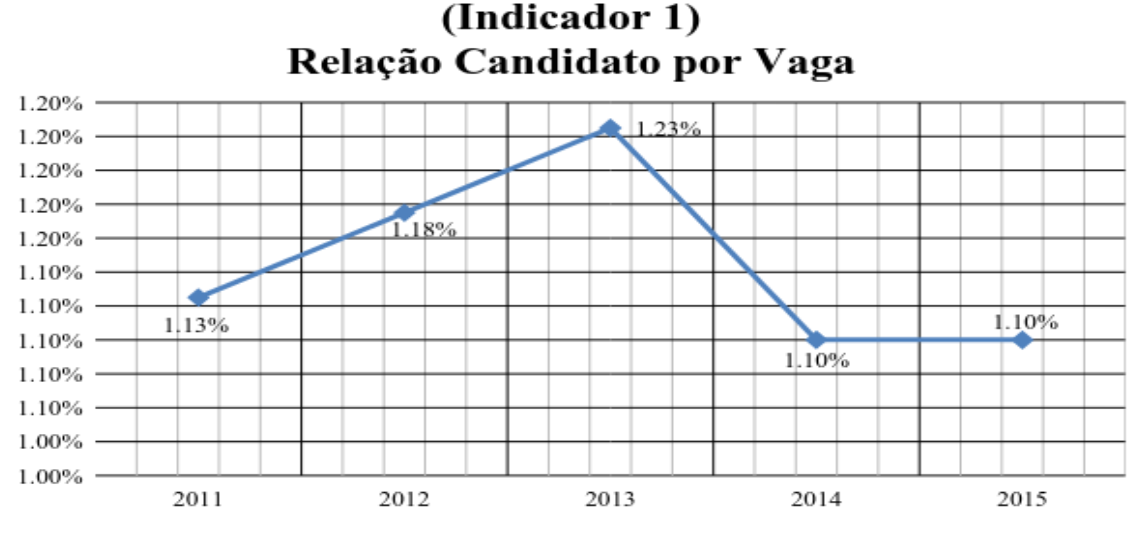
\includegraphics[width=.9\linewidth]{PIP-97-1}
	\end{figure}
	
	O indicador 2 mostra a relação de ingresso por matrícula atendida, este indicador mede a
	capacidade de renovação do quadro discente do campus, como exemplo desse indicador
	apresentamos o Curso de Agronomia do Campus de Colorado do Oeste onde, no segundo
	semestre de 2011, houve um índice de mais de 95\% na quantidade de matrículas efetivadas,
	porém nos anos seguintes esse índice entrou em queda, tendo no primeiro semestre de 2012 uma
	queda de 40\% se comparado ao semestre anterior e, no segundo semestre de 2012, essa redução
	foi de 60\% se comparado ao ano anterior. Nota-se que, nos anos seguintes, a taxa de ingresso
	continuou caindo, se formos comparar o ano que teve a maior taxa de matrícula (2011/2) com o
	último ano analisado (2015/2) a diferença foi de pouco mais de 84\%, tendo esse ultimo ano pouco
	mais de 11\% de ingressantes.
	Este indicador é o resultado da equação ingressantes / matrícula atendida. Sendo assim, o ponto
	fora da curva apresentado pelo dado do ano de 2011/2 (95\%), decorre do fato de que não há
	parâmetro comparativo com anos anteriores, de modo que o divisor para este cálculo (matrícula
	atendida = 0), sendo necessário então, desconsiderar aqueles valores para uma análise mais
	precisa, considerando, portanto, apenas a linha mais estável.
	
	\begin{figure}[ht]
		\centering
		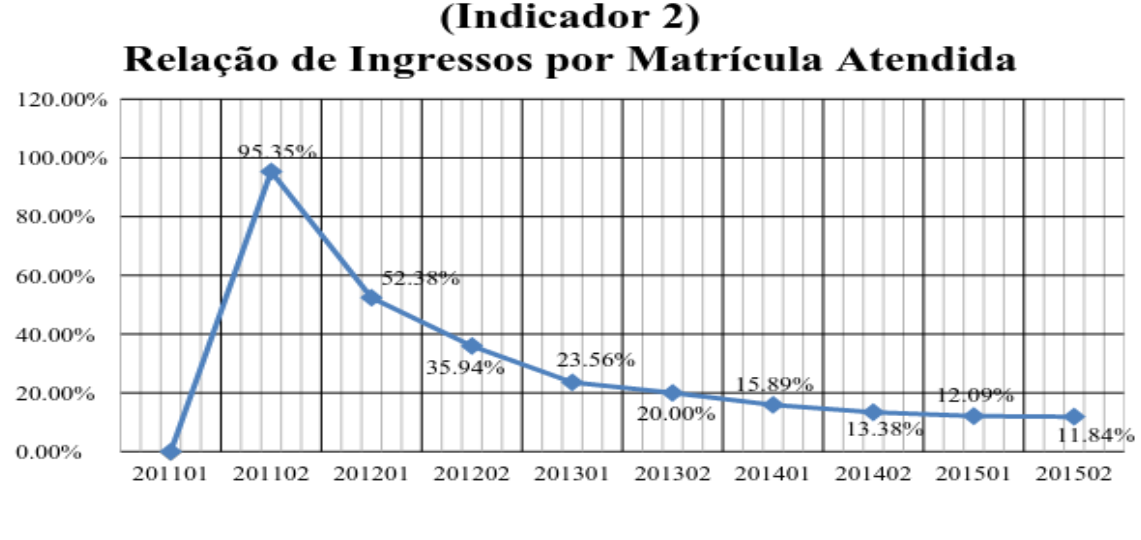
\includegraphics[width=.9\linewidth]{PIP-97-2}
	\end{figure}
	
	O indicador 3 mostra a relação de concluintes por matrícula atendida Esse indicador mede
	a relação entre o total dos alunos matriculados e os que concluíram o curso no tempo previsto,
	mensurando a capacidade de alcançar êxito escolar. Exemplo desse indicador é o do Curso de
	Licenciatura em Química do Campus de Ji-Paraná onde no primeiro ano da análise (2010) o índice de concluintes no tempo previsto foi pouco mais de 30\%, caindo para cerca de 16\% no ano
	seguinte (2011) e, nos anos de 2012 a 2015, não sendo possível analisar a sequencia deste
	indicador, visto que os ciclos de matrículas subsequentes ainda não haviam sido integralizados no
	momento da extração da base de dados para esta análise.
	
	\begin{figure}[ht]
		\centering
		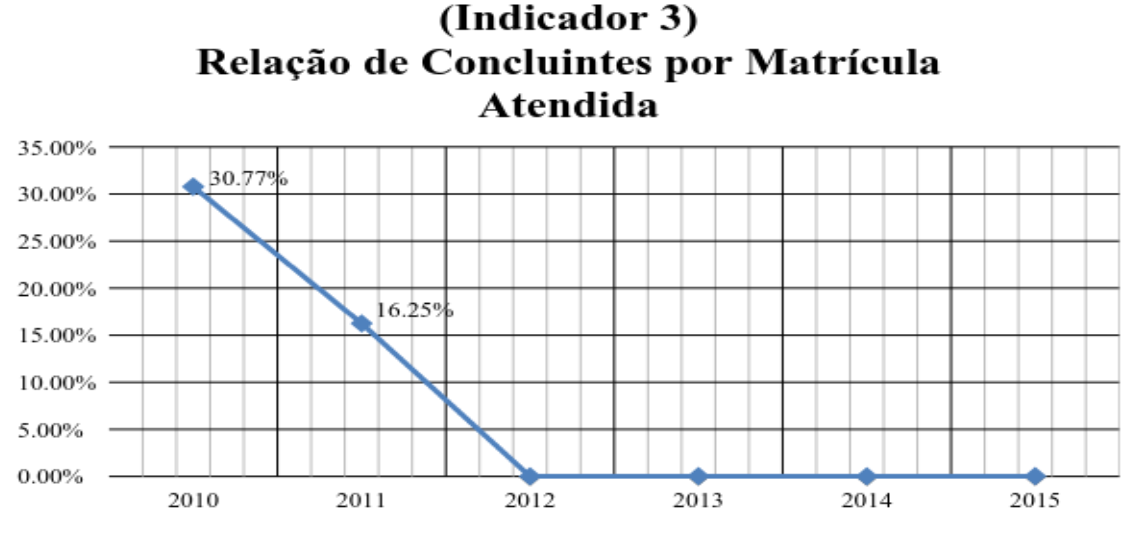
\includegraphics[width=.9\linewidth]{PIP-97-3}
	\end{figure}
	
	O indicador 4 mostra a eficiência acadêmica de concluintes. Esse indicador mede a relação
	entre todos os alunos que concluíram o curso no período previsto e todos que de alguma forma
	finalizaram o curso (desistências/evasões/trancamentos/transferências e desligamentos). Exemplo
	desse indicador é o do Curso de Gestão Pública do Campus Porto Velho Zona Norte onde nos 3
	anos que foram analisados (2013-2015), como demonstra o gráfico abaixo, somente no ano de
	2013 há dados para serem analisados. O índice de êxito em 2013 foi de pouco mais de 26\%. Já
	nos anos 2014 e 2015 essas taxas ainda estão em zero porque os alunos ainda estavam em curso.
	
	\begin{figure}[ht]
		\centering
		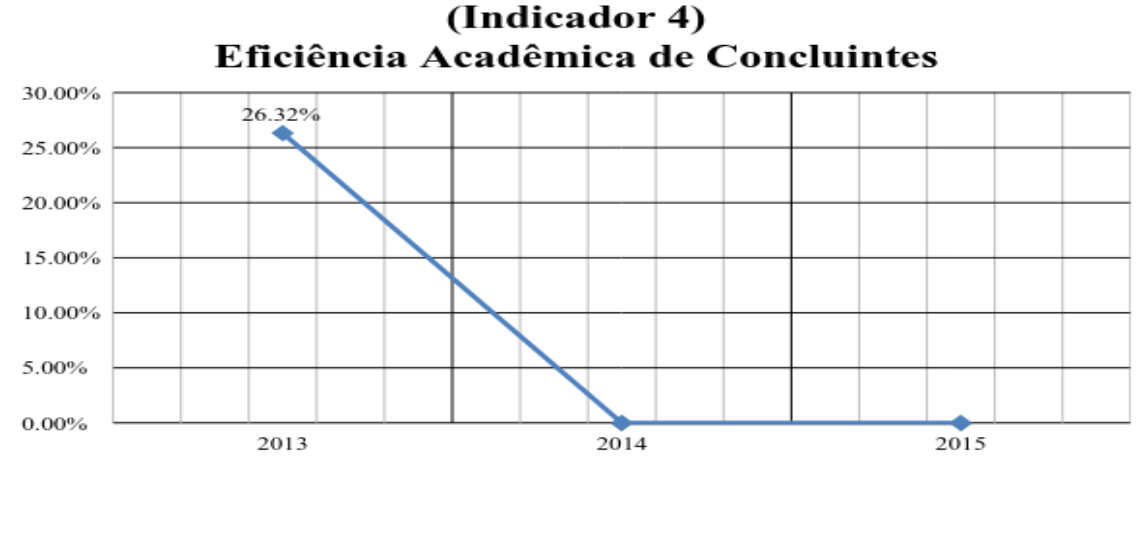
\includegraphics[width=.9\linewidth]{PIP-97-4}
	\end{figure}

	O indicador 5 mostra a retenção do fluxo escolar. Esse indicador mede a relação de alunos
	que não concluíram o curso no tempo previsto. Exemplo desse indicador é o Curso de
	Licenciatura em Química do Campus Ji-Paraná onde, no ano de 2010, o índice de retenção foi
	pouco mais de 12\%, sendo que em 2011 subiu para pouco mais de 22\%. No período de 2012 a
	2015 essa taxa de retenção foi para zero devido esses alunos ainda estarem cursando.
	
	\begin{figure}[ht]
		\centering
		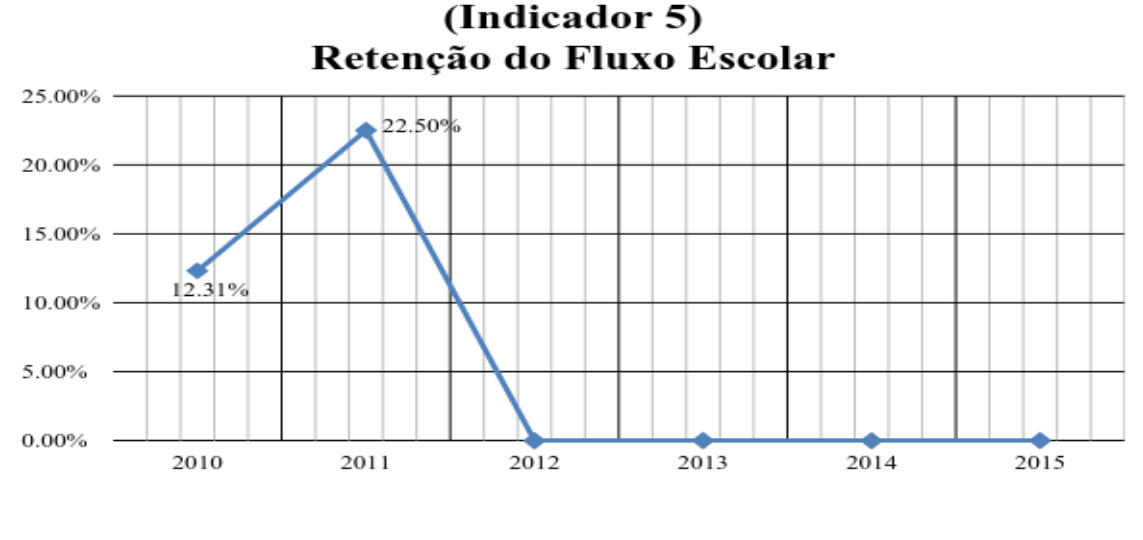
\includegraphics[width=0.7\linewidth]{PIP-97-5}
	\end{figure}
	
	Nota-se, a partir dos resumos apresentados acima, onde cada curso escolhido apresentou um
	ou mais indicadores, que há variações no desempenho de cada curso, decorrente de variáveis
	locais, regionais, pedagógicas e curriculares, determinando assim, as variáveis observadas tanto no desempenho acadêmico quanto no desempenho institucional.
	
	Os processos de evasão, retenção, transferências e desligamentos constituem o rol de
	indicadores negativos dos cursos e da instituição, cujos, dependendo do grau que se apresentam,
	conduzem a necessidade de reformulações. Por outro lado, a aderência da oferta aos Arranjos
	Produtivos Locais e às demandas das comunidades onde se inserem os cursos analisados, bem
	como os índices de permanência e êxito observados em determinados cursos, conduzem a análise
	da assertividade das ofertas.
	
	\section*{Discussões}
	No contexto do planejamento estratégico que envolve tanto o diagnóstico quanto o
	monitoramento e a tomada de decisão das realidades que se deseja transformar, a gestão das
	políticas públicas passou a receber uma medição sistemática por meio de indicadores que são
	definidos como ferramentas “[...] que podem contribuir para a realização de monitoramento e
	avaliação eficazes”. (BRASIL, 2012).
	
	Os indicadores de desempenho, termo utilizado no âmbito da administração, são
	ferramentas utilizadas para o gerenciamento do sistema organizacional e são importantes na
	medida em que fomentam o diálogo, balizam decisões, avaliam iniciativas e induzem melhorias
	ao criarem referência. Os indicadores constituem-se de uma linguagem matemática que
	parametriza referências com a finalidade de medir a eficiência, eficácia e a efetividade de
	processos organizacionais. Desse modo, os indicadores são definidos como um valor quantitativo
	produzido a partir de um período de tempo que permite adquirir informações sobre atributos,
	características e resultados de um serviço, produto, sistema ou processo específico.
	
	Uma dos pontos positivos desse projeto é que seus dados possibilitarão a autoavaliação institucional. Segundo Eloi (2015) constitui-se em um processo de autoconhecimento que
	dinamiza uma análise crítica da prática pedagógica e administrativa de uma instituição
	educacional.
	
	A importância da avaliação institucional deve ser considerada pela instituição, pois ela
	influencia diretamente no cotidiano escolar. Uma boa avaliação institucional terá “[...]
	consequências positivas para o nível de avaliação da aprendizagem em sala de aula” (FREITAS
	et, al. 2014, p.44). Observa-se que a função do planejamento é a mais importante do processo
	administrativo, pois ela sustenta a estratégia da instituição que poderá organizar seus recursos,
	coordenar seus esforços para atingir a sua visão de futuro.
	
	A composição das instituições que atualmente formam a Rede de Educação Profissional,
	Científica e Tecnológica é resultado da integração de 19 escolas de aprendizes artífices instituídas
	por um decreto presidencial de 1909, assinado por Nilo Peçanha, que posteriormente foram
	transformadas nos liceus industriais, depois escolas industriais e técnicas quando da incorporação
	do ensino profissional ao ensino médio e, finalmente, nas famosas escolas técnicas federais
	quando tornarem-se autarquias em 1959.
	
	Nesse percurso também foram constituídas as Escolas Agrotécnicas Federais, seguindo o
	modelo escola-fazenda e com vinculação ao Ministério da Agricultura, posteriormente assumidas
	pelo Ministério da Educação e Cultura em 1967, sendo a partir de então denominadas de escolas
	agrícolas. Na final da década de 1970 mais uma mudança. A transformação de três escolas
	federais1
	em centros federais de educação tecnológica (CEFETs) demarcou uma importante
	mudança na identidade originária dessa rede que foi a equiparação da educação superior aos
	centros universitários.
	
	Uma das características inerentes aos Institutos Federais com relação a sua configuração
	organizacional e espacial é o fato de ser multicampi o que lhes confere vantagens e desvantagens.
	Para Paiva (2015) um dos benefícios caracterizou-se pela ampliação do acesso de indivíduos à
	educação, mas com algumas dificuldades , dentre elas a dispersão geográfica entre as unidades
	exigindo uma gestão diferenciada que possibilitasse a comunicação e a integração institucional. 
	
	Bueno (2015) destaca que para se implantar um curso no Instituto Federal, “é necessário o
	conhecimento da demanda local para que em seguida possa se estabelecer o eixo tecnológico e
	assim criar cursos a serem trabalhados nos diversos níveis e modalidades de ensino” (p.128).
	
	Assim, o levantamento de dados educacionais é importante para traçar um perfil da
	instituição, conhecer seus pontos fortes e limitações, gerando indicadores acadêmicos que
	fornecem aos gestores das instituições de ensino informações imprescindíveis ao processo de
	tomada de decisões e servindo de subsidio para a formulação de políticas públicas na área da
	educação.
	
	\subsection*{NOTA DOS PESQUISADORES}
	Com a finalidade de instrumentalizar a análise, por meio da padronização no uso de termos e
	conceitos, destacamos abaixo o conceito das diferentes situações em que os estudantes podem
	estar durante o curso:
	
	\textbf{a) Vagas Ofertadas:} é o total de vagas ofertadas para o curso naquele período/semestre;
	
	\textbf{b) Matrículas Iniciais:} é a quantidade de alunos matriculados naquele período/semestre;
	
	\textbf{c) Em curso/retidos:} é aquela matrícula que permanece com situação em “curso” tendo já
	finalizado o período de duração do curso;
	
	\textbf{d) Transferência Externa:} todo aquele aluno que está sendo transferido para outra unidade
	federal ou outra rede de ensino;
	
	\textbf{e) Integralizado:} aquele aluno que concluiu os componentes curriculares, mas que ainda
	não está apto a colar grau ou que ainda não concluiu alguma pendência curricular;
	
	\textbf{f) Desligado:} é todo aluno que por algum motivo trancou o curso;
	
	\textbf{g) Evadido:} é todo aluno, que desistiu do curso, sem formalizar a desistência e
	
	\textbf{h) Concluído:} todos que terminaram o curso com êxito independente do período.
	
	Os dados analisados neste trabalho referem-se à extração realizada pelo Sistema Nacional de
	Informações da Educação Profissional e Tecnológica (SISTEC)
	2
	no dia 26 de setembro de 2016
	as 16h09min. Como o sistema é aberto aos agentes da Coordenação de Registro Acadêmico
	(CRA) para atualização contínua com base no fluxo de estudantes, se utilizarmos os mesmos
	parâmetros de pesquisa, cálculo e coleta de dados, é possível chegar a conclusões diferentes,
	dependendo do período em que a extração foi realizada. Assim, os resultados analisados a seguir
	se referem ao período até o momento em que os dados foram extraídos e, consideram somente os
	dados inseridos pelos agentes das CRA’s do IFRO desde o início do registro. Além disso,
	alertamos para o fato de que a análise se refere aos cursos com ciclos concluídos.
	
	A decisão pela análise dos cinco (05) indicadores decorre do fato de que com eles é possível
	verificar o processo de desenvolvimento da educação profissional e tecnológica ofertado pelo
	IFRO a partir das abordagens da aderência da oferta de cursos com os APLs e com as demandas
	das comunidades (Indicador de Candidato x Vaga e ingresso x aluno); é possível verificar o
	processo(as intercorrências da dinâmica interna do curso), a partir da análise dos indicadores
	(Retenção do Fluxo Escolar e ingressante x matrícula atendida), observando a capacidade de
	renovação do corpo discente, e, é possível verificar a eficiência do curso e da instituição a partir
	da análise do indicador de (eficiência de concluintes).
	
	\subsection*{ANÁLISE}

	\begin{figure}[ht]
		\centering
		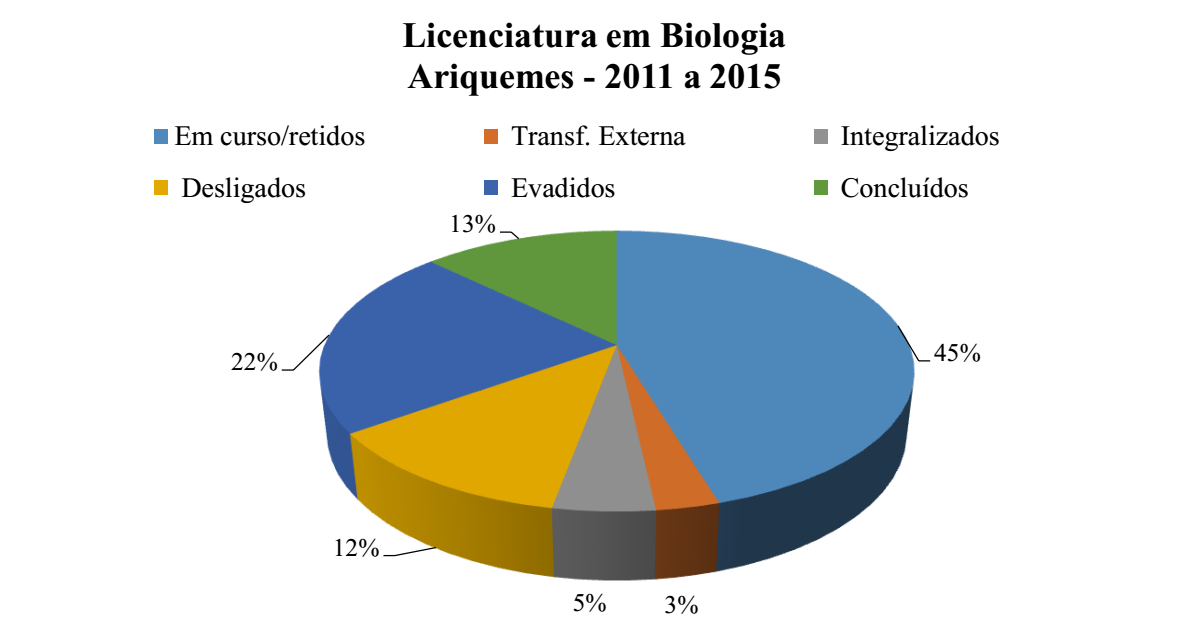
\includegraphics[width=.8\linewidth]{pip-97-6}
	\end{figure}
	Os dados representados no gráfico referem-se ao acumulado de matrículas iniciais durante o
	período observado (2011 a 2015).
	Observa-se que no curso de licenciatura em Biologia no campus de Ariquemes quase a
	metade dos alunos acabam retidos mesmo já tendo finalizado o período de duração de seu curso.
	Isso quer dizer, nesse caso específico, que 45\% dos alunos matriculados no curso de licenciatura
	em Biologia não irão formar-se no tempo previsto do curso que é de 4 anos. Nota-se também que 37\% do total de alunos matriculados, acabam desistindo, transferindo ou trancando o curso. A
	conclusão de alunos neste curso é de 13\% do total de alunos matriculados inicialmente.
	
	\begin{figure}[ht]
		\centering
		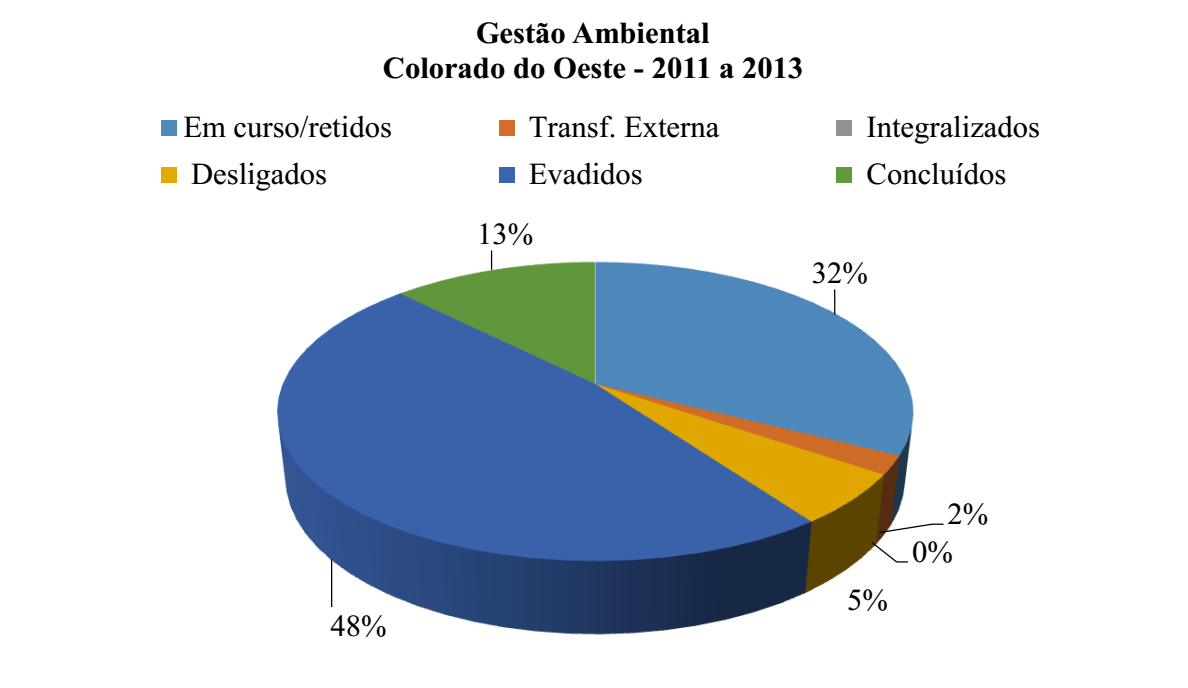
\includegraphics[width=.8\linewidth]{pip-97-7}
	\end{figure}

	Os dados representados no gráfico referem-se ao acumulado de matrículas iniciais durante o
	período observado (2011 a 2013).
	Observa-se que mais da metade (52\%) dos alunos matriculados inicialmente no curso de
	Gestão Ambiental no Campus Colorado do Oeste acabam desistindo, transferindo ou trancando o
	curso neste campus, fora isso 32\% dos alunos acabam ficando retidos no curso e não concluindo o
	curso no período previsto de duração do curso.
	A quantidade de alunos que conclui é de 13\% do total de matriculados inicialmente.
	
	\begin{figure}[ht]
		\centering
		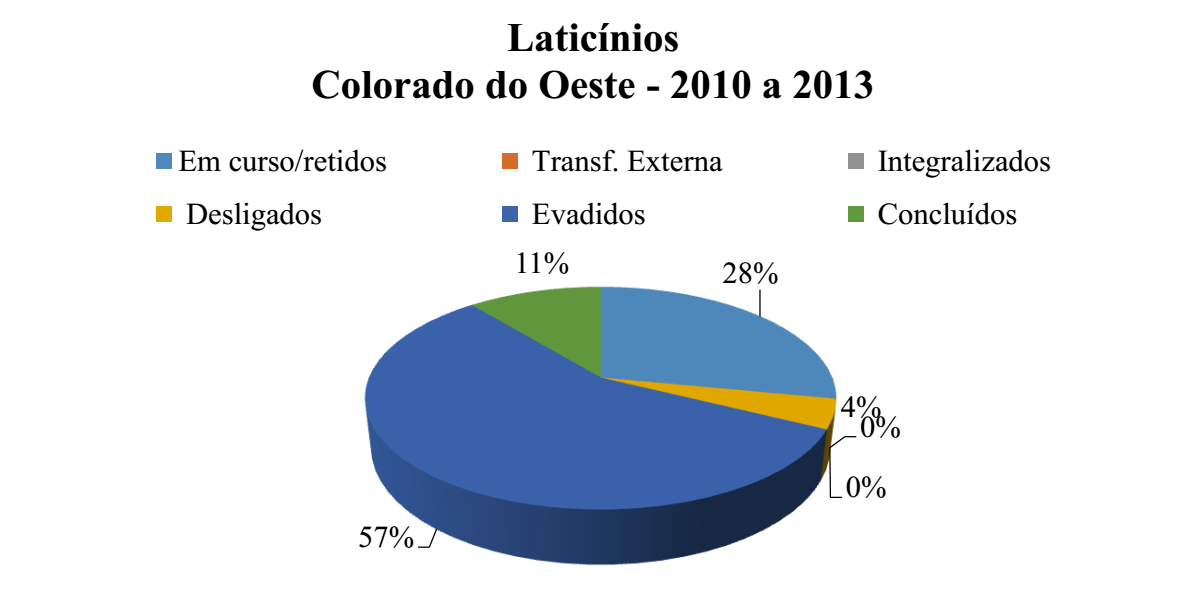
\includegraphics[width=.8\linewidth]{pip-97-8}
	\end{figure}
	
	Os dados representados no gráfico referem-se ao acumulado nas matrículas iniciais durante
	o período observado (2010 a 2013).
	
	Nota-se que 61\% dos alunos matriculados inicialmente no curso de Laticínios no Campus
	de Colorado do Oeste acabam desistindo ou trancando o curso, além dos 28\% que não irão
	concluir o curso no tempo previsto de duração e tendo apenas 11\% de conclusão do total de
	alunos matriculados inicialmente.
	
	\begin{figure}[ht]
		\centering
		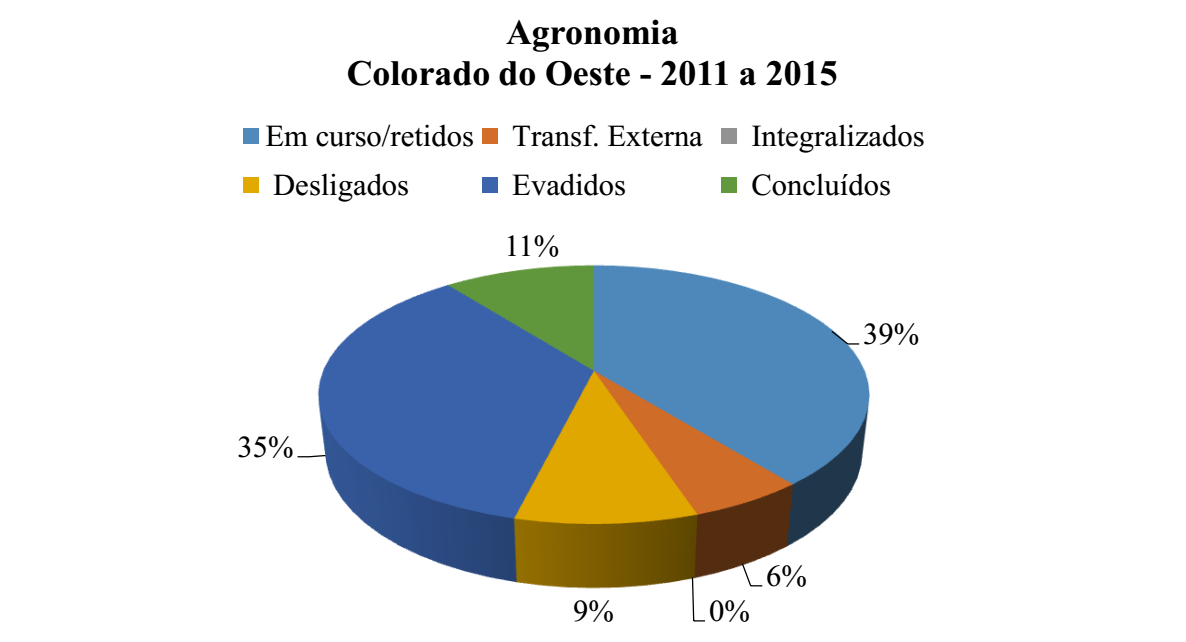
\includegraphics[width=0.8\linewidth]{pip-97-9}
	\end{figure}
	
	Os dados representados no gráfico referem-se ao acumulado nas matrículas iniciais durante
	o período observado (2011 a 2015).
	
	Observa-se no curso de Agronomia de Colorado do Oeste que 50\% dos alunos matriculados
	inicialmente no curso acabam sendo desligados, evadidos ou transferidos, além disso, 39\% dos
	alunos matriculados inicialmente acabam ficando retidos, isto é, não irão concluir o curso no
	tempo previsto.
	
	A taxa de conclusão no curso de Agronomia é de 11\% do total de alunos matriculados
	inicialmente.
	
	\begin{figure}[ht]
		\centering
		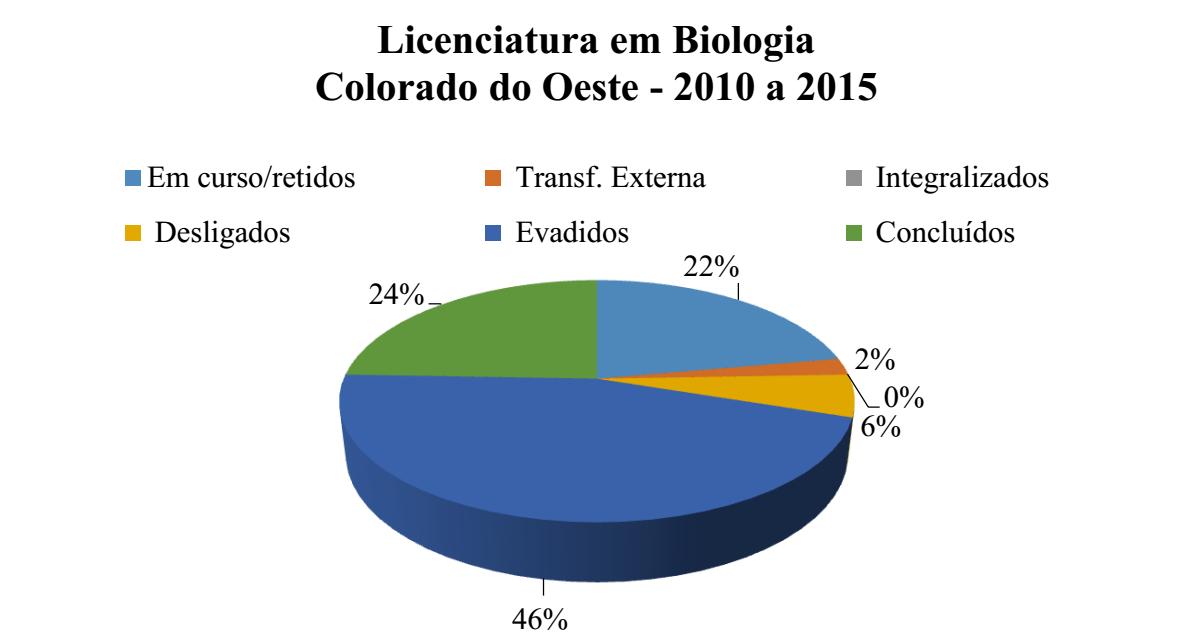
\includegraphics[width=0.8\linewidth]{pip-97-10}
	\end{figure}
	
	Os dados representados no gráfico referem-se ao acumulado nas matrículas iniciais durante o
	período observado (2010 a 2015).
	
	O curso de licenciatura em Biologia do Campus Colorado do Oeste teve, no período
	analisado, 54\% de alunos desligados, evadidos ou com transferência externa, tendo as matrículas
	iniciais como base.
	
	Os alunos retidos no curso são de 22\%, o que significa dizer que 22\% dos alunos não irão
	concluir o curso no tempo previsto. 24\% dos alunos matriculados inicialmente obtiveram êxito
	em concluir o curso.
	
	\begin{figure}[ht]
		\centering
		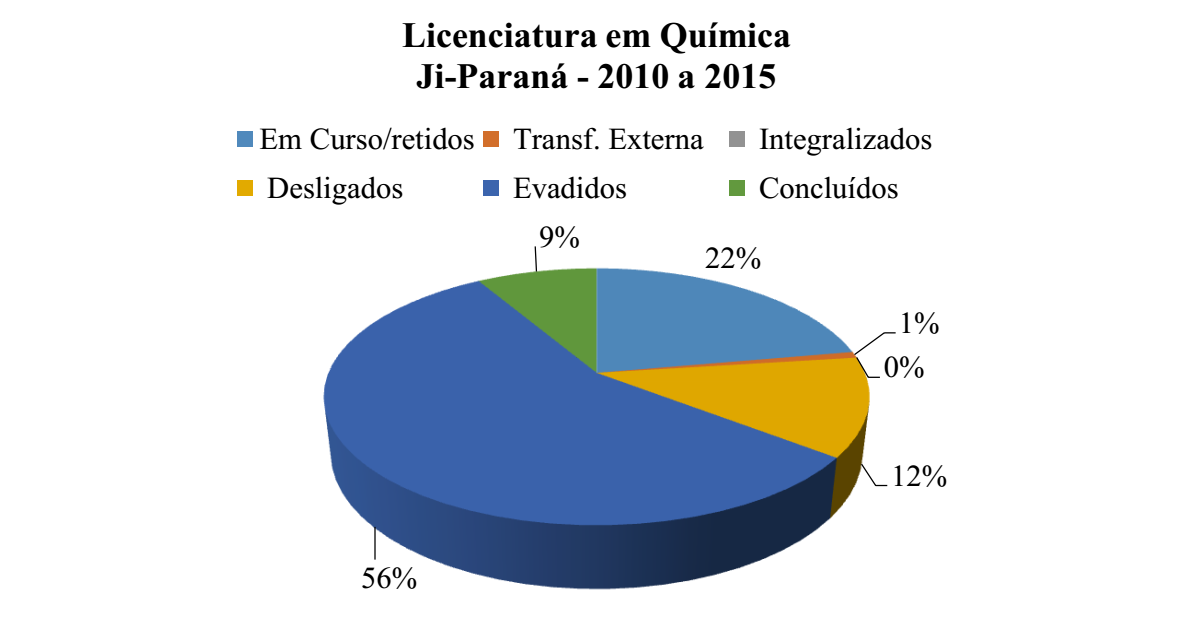
\includegraphics[width=0.8\linewidth]{pip-97-11}
	\end{figure}
	
	Os dados representados no gráfico referem-se ao acumulado nas matriculam iniciais
	durante o período observado (2010 a 2015).
	
	Nota-se que no Campus Ji-Paraná 69\% dos alunos matriculados inicialmente acaba
	trancando, transferindo ou evadindo-se do curso de licenciatura em Química. Outros 22\% acabam
	não concluindo o curso no tempo previsto e somente 9\% dos alunos matriculados inicialmente no
	curso acabam concluindo o curso com êxito.
	
	\begin{figure}[ht]
		\centering
		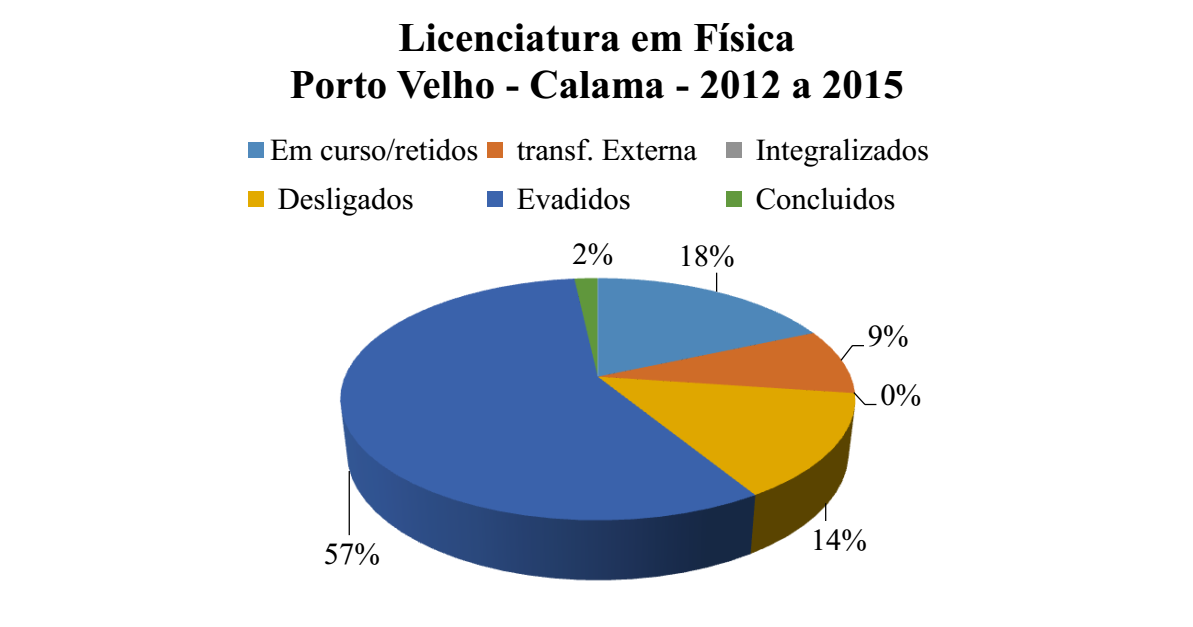
\includegraphics[width=0.8\linewidth]{pip-97-12}
	\end{figure}
	
	Os dados representados no gráfico referem-se ao acumulado nas matrículas iniciais durante o
	período observado (2012 a 2015).
	
	Observa-se que o curso de licenciatura em Física do campus Porto Velho – Calama 80\% dos
	alunos matriculados inicialmente acaba trancando, transferindo ou evadindo-se do curso, além dos
	18\% de alunos que acabam ficando retidos, isso significa que não irão formar-se no tempo
	previsto do curso.
	
	A taxa de alunos matriculados inicialmente que se formam é somente de 2\%.
	
	\begin{figure}[ht]
		\centering
		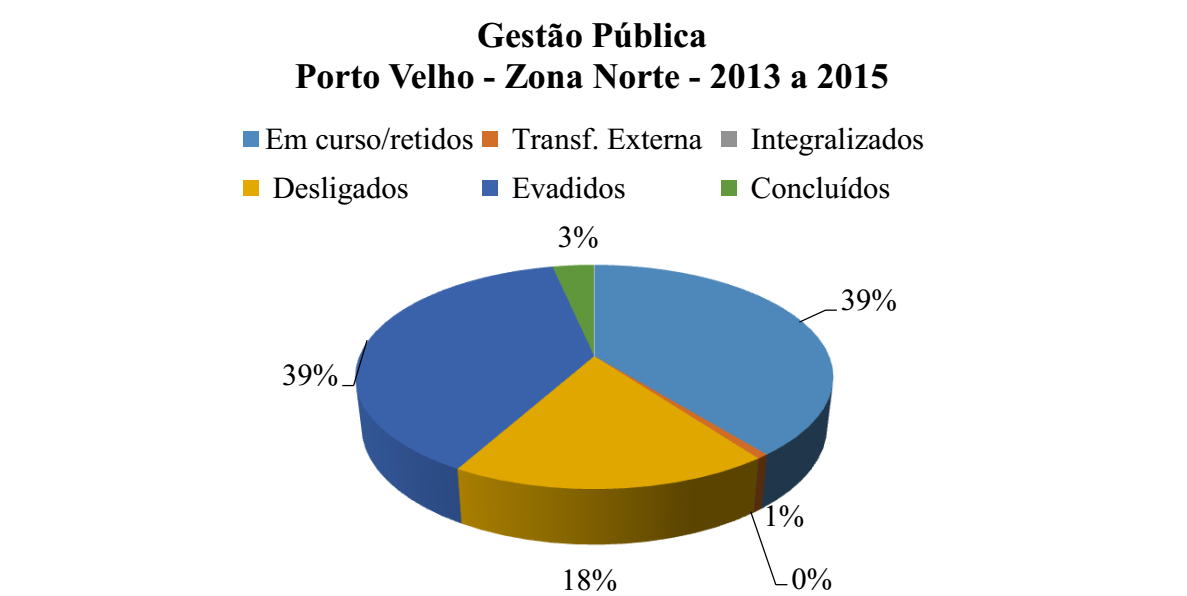
\includegraphics[width=0.8\linewidth]{pip-97-13}
	\end{figure}
	
	Os dados representados no gráfico referem-se ao acumulado nas matrículas iniciais durante o
	período observado (2013 a 2015).
	
	No curso de Gestão Pública do campus Porto Velho Zona Norte 58\% de alunos acaba
	desistindo, trancando ou transferindo de curso e 38\% dos matriculados inicialmente são retidos,
	isso significa que não irão formar-se no tempo previsto do curso.
	
	Apenas 3\% dos alunos matriculados inicialmente concluem o curso.
	
	\begin{figure}[ht]
		\centering
		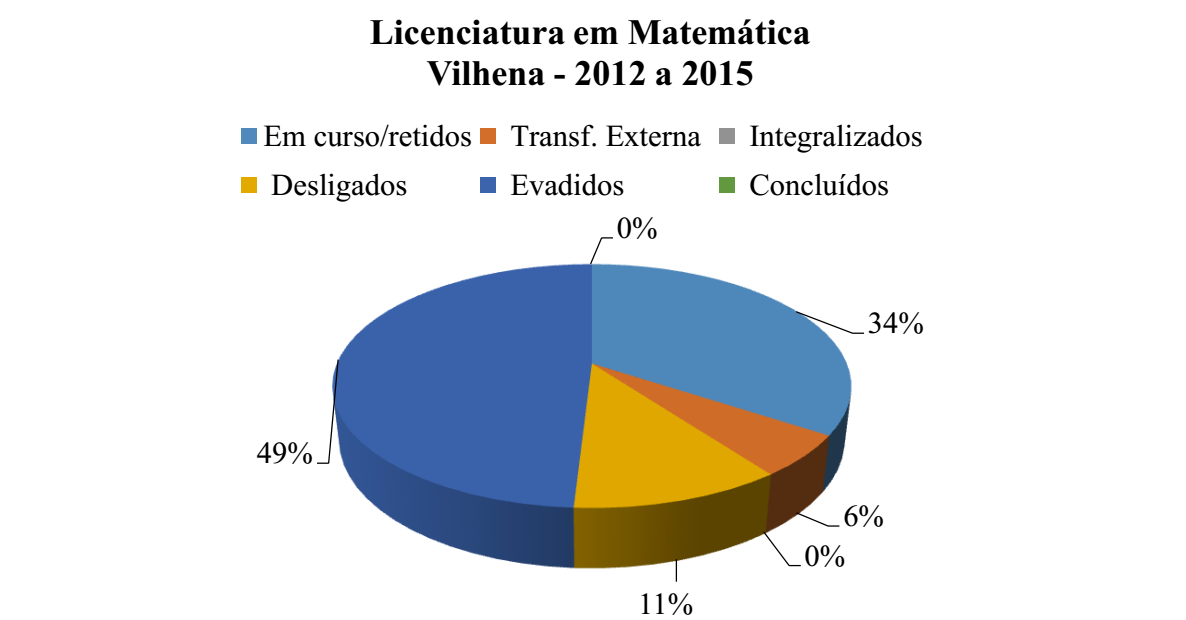
\includegraphics[width=0.8\linewidth]{pip-97-14}
	\end{figure}
	
	Os dados representados no gráfico referem-se ao acumulado de matrículas iniciais durante
	o período observado (2012 a 2015).
	
	Nota-se que 66\% dos alunos matriculados inicialmente acabam evadindo-se, desligando-se
	ou transferindo-se do curso de licenciatura em Matemática do campus de Vilhena, além dos 34\%
	de alunos matriculados inicialmente que acabam ficando retido no curso. Isso significa dizer que
	não conseguiram concluir o curso no tempo previsto inicialmente. E a taxa de conclusão até a data
	de coleta dos dados foi de 0\% (é provável que o sistema não tenha sido atualizado no período
	correto).
	
	\subsubsection*{Dados dos Cursos de Graduação do IFRO}
	
	\begin{figure}[ht]
		\centering
		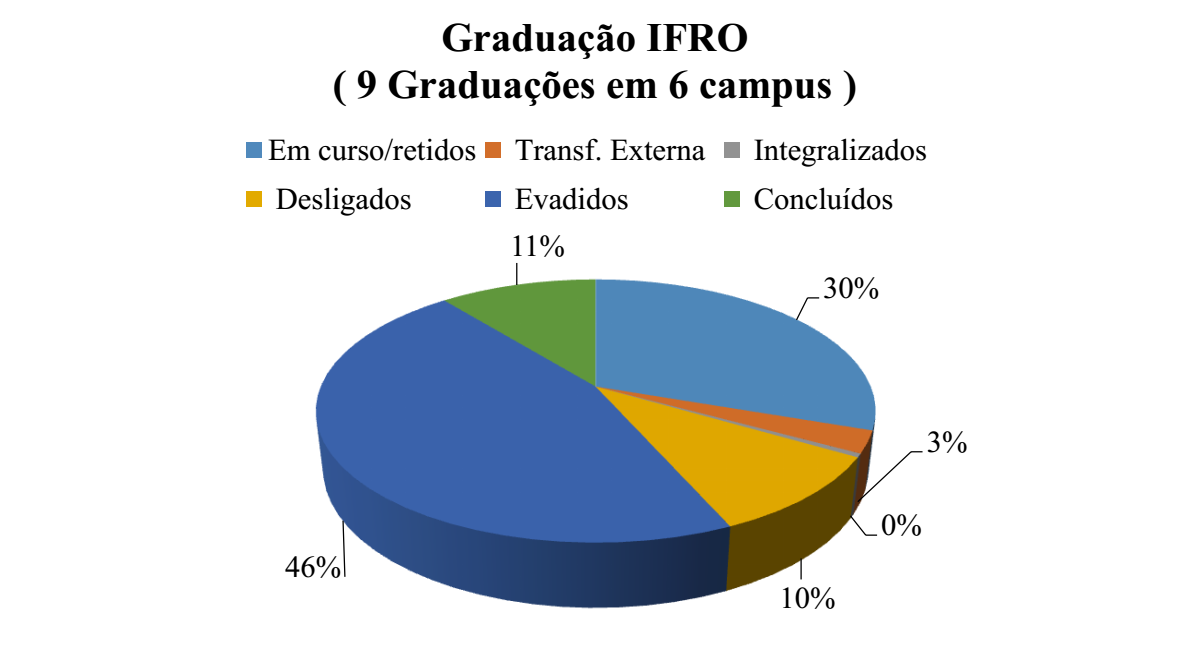
\includegraphics[width=0.8\linewidth]{pip-97-15}
	\end{figure}
	
	Os dados avaliados referem-se à amostra de 9 (nove) cursos de graduações, o critério
	utilizado pela a seleção da amostra foi o fato de que a amostra selecionada possuía ciclos de
	matriculas finalizados na data da coleta dos dados no sistema SISTEC, sendo distribuídos em 6
	(seis) campus pelo estado, sendo 5 (cinco) Licenciaturas, 1(um) bacharelado e 3 (três) tecnólogos.
	O IFRO até a data da coleta dos dados disponibilizou 1960 (mil novecentos e sessenta) vagas para
	graduação, tendo matriculado no total 2381 (dois mil trezentos e oitenta e um) alunos,
	distribuídos em 1080 (mil e oitenta) vagas para licenciatura, 400 (quatrocentos) vagas para
	bacharelado e 480 (quatrocentos e oitenta) vagas para tecnólogo. A taxa de graduação observada
	foi 59\% dos alunos matriculados inicialmente acabam que desistindo, trancando ou transferindo-
	se de instituição, 30\% acabaram ficando retido na graduação, isso significa que não irão colar
	grau no tempo previsto de cada curso e 11\% dos alunos matriculados inicialmente concluem a
	graduação.
	
	\section*{SÍNTESE DOS RESULTADOS}
	
	1. Os dados analisados neste trabalho referem-se à extração realizada pelo Sistema Nacional
	de Informações da Educação Profissional e Tecnológica (SISTEC)3 no dia 26 de setembro de 2016 as 16h09min.
	
	2. Os dados avaliados referem-se à amostra de 9 (nove) cursos de graduação. O critério
	utilizado para a seleção da amostra foi seleção de cursos com ciclos de matrícula
	finalizados na data da coleta dos dados no sistema SISTEC, distribuídos em 6 (seis)
	campus pelo estado, sendo 5 (cinco) Licenciaturas, 1(um) bacharelado e 3 (três)
	tecnólogos.
	
	3. O IFRO, até a data da coleta dos dados, disponibilizou 1960 (mil novecentos e sessenta)
	vagas para graduação, tendo matriculado no total 2381 (dois mil trezentos e oitenta e um)
	alunos, distribuídos em 1080 (mil e oitenta) vagas para licenciatura, 400 (quatrocentos)
	vagas para bacharelado e 480 (quatrocentos e oitenta) vagas para tecnólogo.
	
	4. Nos cursos de graduação, 59\% dos alunos matriculados inicialmente acabam desistindo,
	trancando ou transferindo-se para outra instituição;
	
	5. Nos dados consolidados de todas as unidades, constatou-se nos cursos de graduação um
	alto índice de retenção do fluxo escolar (30\% );

	6. Na análise dos microdados, constatou-se:
	
	7. No curso de \textbf{Licenciatura em Biologia no Campus de Ariquemes} quase a metade dos
	alunos acabam retidos, mesmo já tendo finalizado o período de duração de seu curso;
	
	8. Mais da metade (52\%) dos alunos matriculados inicialmente no \textbf{Curso de Gestão
	Ambiental no Campus de Colorado do Oeste} acabam desistindo, transferindo ou
	trancando o curso e 32\% dos alunos acabam ficando retidos e não concluindo o curso no
	período previsto;
	
	9. Constatou-se que 61\% dos alunos matriculados inicialmente no \textbf{Curso de Laticínios no
	Campus de Colorado do Oeste} acabam desistindo ou trancando o curso, além dos 28\%
	que não irão concluir o curso no tempo previsto de duração e tendo apenas 11\% de
	conclusão do total de alunos matriculados inicialmente;
	
	10. \textbf{No Curso de Agronomia do Campus Colorado do Oeste} que 50\% dos alunos
	matriculados inicialmente acabam sendo desligados, evadidos ou transferidos, 39\% dos
	acabam ficando retidos, isto é, não irão concluir o curso no tempo previsto;
	
	11. O \textbf{Curso de Licenciatura em Biologia do Campus Colorado do Oeste} teve, no período
	analisado, 54\% de alunos desligados, evadidos ou com transferência externa, tendo as
	matrículas iniciais como base e 22\% dos alunos não irão concluir o curso no tempo
	previsto. O índice de êxito escolar é de 24\%;
	
	12. No \textbf{Campus Ji-Paraná} 69\% dos alunos matriculados inicialmente acaba trancando,
	transferindo ou evadindo-se do \textbf{Curso de Licenciatura em Química}. Outros 22\% acabam
	não concluindo o curso no tempo previsto e somente 9\% dos alunos matriculados
	inicialmente no curso acabam concluindo o curso com êxito;
	
	13. Observa-se que o\textbf{ Curso de Licenciatura em Física do Campus Porto Velho – Calama}
	80\% dos alunos matriculados inicialmente acaba trancando, transferindo ou evadindo-se
	do curso, além dos 18\% que ficam retidos, isso significa que não irão formar-se no tempo
	previsto para o curso. A taxa de alunos matriculados inicialmente que se forma é somente
	de 2\%.
	
	14. No \textbf{Curso de Gestão Pública do Campus Porto Velho Zona Norte} 58\% de alunos
	acaba desistindo, trancando ou se transferindo de curso e 38\% dos matriculados
	inicialmente são retidos, isso significa que não irão formar-se no tempo previsto do curso.
	Apenas 3\% dos alunos matriculados inicialmente concluem o curso.
	
	15. 66\% dos alunos matriculados inicialmente acabam evadindo-se, desligando-se ou
	transferindo-se do curso de \textbf{Licenciatura em Matemática do Campus de Vilhena}, além
	dos 34\% de alunos matriculados inicialmente retidos. A taxa de conclusão até a data de
	coleta dos dados foi de 0\% (é provável que o sistema não tenha sido atualizado no período
	correto).
	
	16. No IFRO, apenas 11\% dos alunos matriculados inicialmente, concluem a graduação.
	
	\section*{Referências}
	\sloppy
	\noindent BUENO, Daniela Gomes Martins. \textbf{Institutos Federais de Educação, Ciência e Tecnologia:}
	uma política a ser cravada na história. Curitiba: Appris, 2015.
	
	\noindent BRASIL. Ministério da Educação. \textbf{Manual para Produção e Análise dos Indicadores da
	Rede Federal de EPCT}. Acórdão TCU no 2.267/2005. Exercício 2014. Janeiro de 2015
	http://sitesistec.mec.gov.br/images/arquivos/pdf/manual\_indicadores\_gestao\_exercicio2014.pdf.
	Acesso em 08 de maio de 2016.
	
	\noindent ELOI, Merilande. \textbf{Avaliação institucional nos campos dos Institutos Federais:} uma proposta
	para atendimento da Educação Profissional Técnica de Nível Médio do Instituto Federal
	Baiano. Jundiaí: Paco Editorial, 2015.
	
	\noindent FREITAS, Luiz Carlos de et. al. \textbf{Avaliação educacional:} caminhando pela contramão. 7 ed.
	Petrópolis, RJ:Vozes,2014. (Col. Fronteiras educacionais).
	
	\noindent INSTITUTO FEDERAL DE EDUCAÇÃO, CIÊNCIAS E TECNOLOGIA DE RONDÔNIA.
	\textbf{Resolução N. 05/CONSUP/IFRO, de 11 de janeiro de 2016.} Dispõe sobre a reformulação do
	Educação, Ciência e Tecnologia de Rondônia. Porto Velho: IFRO, 2016.
	
	\noindent PAIVA, Liz Denize Carvalho. \textbf{Autoavaliação institucional:} perspectivas no âmbito dos
	institutos federais. Curitiba: Appris, 2015.
	
\end{document}
